\documentclass{standalone}
\usepackage{hsbcommon}
\makeatletter\AtBeginDocument{\@buildstepset{total}}\makeatother
\begin{document}
%% Credit in Germany as T-accounts: borrowers (left) and lenders (right).
%% Same machinery as tikz-budgetbars.tex; only the headings differ.
%% Steps: total, households, firms, government
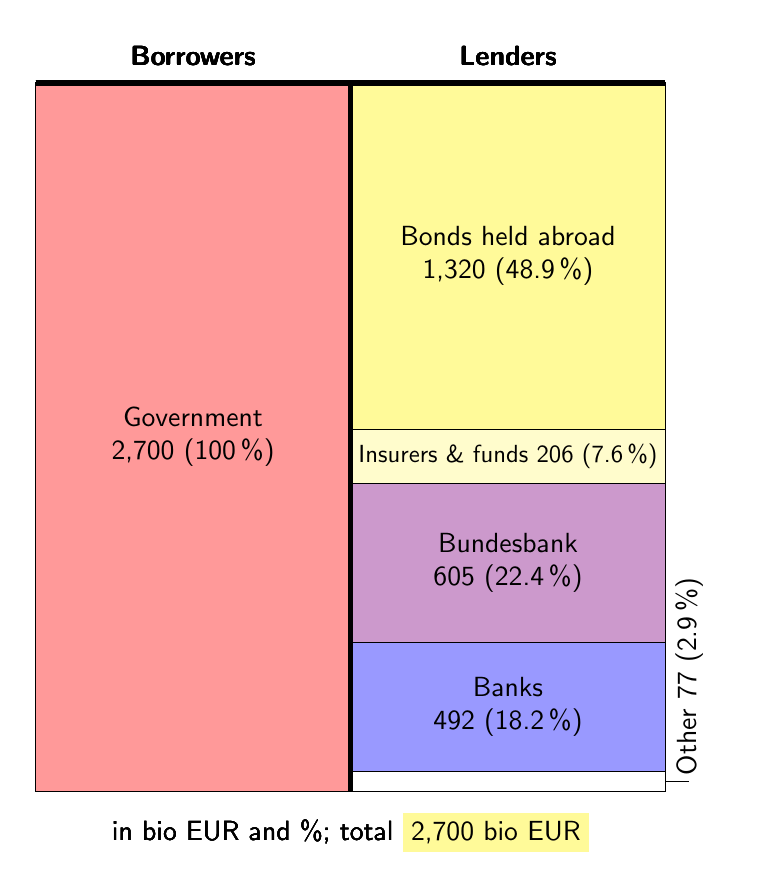
\begin{tikzpicture}
  %%% =================================================================
  %%% LAYOUT (local to this picture; works when \input elsewhere)
  %%% =================================================================
  \def\bdH{9}      % height of the taller bar in cm
  \def\bdW{4}      % bar width in cm
  \def\bdTwo{9}    % segments >= 9 % of the total: name and value on two lines
  \def\bdOne{4.5}  % segments >= 4.5 %: one line; smaller: label outside
  \def\bdRotate{1} % 1: small revenue labels rotated 90 degrees (narrow);
                   % 0: horizontal (use \\ in long names to break them)
  \def\bdShow{3}   % default for the values: 1 absolute, 2 percent, 3 both
                   % (can be overridden per chart: \budgetbars[2]{key})
  \def\bdLeft{Borrowers}   % heading of the left bar
  \def\bdRight{Lenders}    % heading of the right bar
  \tikzset{bd text/.style={font=\sffamily}}
  % \budgetdataset{key}{unit}{total}{borrower list}{lender list}
  % lists: value/color/name, ..., absolute values, stacked from the top down
  \newcommand\budgetdataset[5]{%
    \expandafter\def\csname bd-#1-unit\endcsname{#2}%
    \expandafter\def\csname bd-#1-total\endcsname{#3}%
    \expandafter\def\csname bd-#1-exp\endcsname{#4}%
    \expandafter\def\csname bd-#1-rev\endcsname{#5}}
  % caption below the T-account: #1 unit, #2 total
  \newcommand\bdcaption[2]{%
    \ifcase\bdmode\or in #1\or in \%\or in #1 and \%\fi;
    total \colorbox{yellow!40}{#2 #1}}
  % sum of a list into \bdsum
  \newcommand\bdsumof[1]{%
    \gdef\bdsum{0}%
    \foreach \v/\c/\n in #1 {\pgfmathsetmacro\bdt{\bdsum+\v}\xdef\bdsum{\bdt}}}
  % numbers as printed in the labels
  \newcommand\bdnum[1]{\pgfmathprintnumber[fixed, precision=1, 1000 sep={,}, assume math mode=true]{#1}}
  \newcommand\bdpctof[1]{%
    \pgfmathsetmacro\bdp{#1/\bdsidetotal*100}%
    \pgfmathprintnumber[fixed, precision=1, assume math mode=true]{\bdp}\,\%}
  % value of a segment according to the mode
  \newcommand\bdval[1]{%
    \ifcase\bdmode\or \bdnum{#1}\or \bdpctof{#1}\or \bdnum{#1} (\bdpctof{#1})\fi}
  % shrink a one-line label to the bar width if it is too wide
  \ifdefined\bdbox\else\newsavebox\bdbox\fi
  \newcommand\bdfit[1]{%
    \sbox\bdbox{#1}%
    \pgfmathsetlengthmacro\bdmax{\bdW cm-0.2cm}%
    \ifdim\wd\bdbox>\bdmax\resizebox{\bdmax}{!}{\usebox\bdbox}\else\usebox\bdbox\fi}
  % one segment: #1 x of bar, #2 bottom, #3 top (absolute values), #4 color,
  %              #5 name, #6 value, #7 side for outside labels (-1 left, 1 right)
  \newcommand\bdseg[7]{%
    \pgfmathsetmacro\bdyA{\bdH-#2/\bdscale*\bdH}%   stacked from the top down
    \pgfmathsetmacro\bdyB{\bdH-#3/\bdscale*\bdH}%
    \pgfmathsetmacro\bdyM{(\bdyA+\bdyB)/2}%
    \pgfmathsetmacro\bdpct{#6/\bdscale*100}%
    \draw[fill=#4, draw=black] (#1,\bdyA) rectangle (#1+\bdW,\bdyB);
    \ifdim \bdpct pt<\bdOne pt
      % small segment: no label on the expenditure side; on the revenue side
      % a label outside
      \ifnum#7>0
        \ifnum\bdRotate=1
          % rotated: each label rises from its leader, side by side
          \pgfmathsetmacro\bdxL{#1+\bdW+0.3+\bdcount*0.5}%
          \pgfmathtruncatemacro\bdc{\bdcount+1}\xdef\bdcount{\bdc}%
          \draw (#1+\bdW,\bdyM) -- (\bdxL,\bdyM)
            node[bd text, rotate=90, anchor=west, inner sep=2pt] {#5 \bdval{#6}};
        \else
          \pgfmathsetmacro\bdyL{min(\bdyM,\bdlast-0.45)}%
          \xdef\bdlast{\bdyL}%
          \draw (#1+\bdW,\bdyM) -- (#1+\bdW+0.3,\bdyL)
            node[bd text, anchor=west, align=left] {#5 \bdval{#6}};
        \fi
      \fi
    \else\ifdim \bdpct pt<\bdTwo pt
      \node[bd text] at (#1+\bdW/2,\bdyM) {\bdfit{#5 \bdval{#6}}};
    \else
      \node[bd text, align=center] at (#1+\bdW/2,\bdyM) {#5\\\bdval{#6}};
    \fi\fi
  }
  % one stacked bar: #1 x, #2 list, #3 side for outside labels, #4 heading
  \newcommand\bdbar[4]{%
    \gdef\bdlast{100}\gdef\bdcount{0}%
    \foreach \v/\c/\n [evaluate=\v as \bdtop using \bdbot+\v,
                       remember=\bdtop as \bdbot (initially 0)] in #2 {%
      \bdseg{#1}{\bdbot}{\bdtop}{\c}{\n}{\v}{#3}
    }
    \node[bd text, font=\sffamily\bfseries, anchor=south] at (#1+\bdW/2,\bdH+0.1) {#4};
  }
  % \budgetbars[mode]{key}: borrowers left, lenders right, as a T-account
  %   mode: 1 absolute values, 2 percent of each side's total, 3 both
  \newcommand\budgetbars[2][\bdShow]{%
    \edef\bdmode{#1}%
    \expandafter\let\expandafter\bdexp\csname bd-#2-exp\endcsname
    \expandafter\let\expandafter\bdrev\csname bd-#2-rev\endcsname
    \bdsumof{\bdexp}\let\bdsumE\bdsum
    \bdsumof{\bdrev}\let\bdsumR\bdsum
    \pgfmathsetmacro\bdscale{max(\bdsumE,\bdsumR)}%   both bars on one scale
    \let\bdsidetotal\bdsumE
    \bdbar{-\bdW}{\bdexp}{-1}{\bdLeft}
    \let\bdsidetotal\bdsumR
    \bdbar{0}{\bdrev}{1}{\bdRight}
    \draw[line width=2pt] (0,0) -- (0,\bdH);            % T-account
    \draw[line width=2pt] (-\bdW,\bdH) -- (\bdW,\bdH);
    \node[bd text, anchor=north] at (0,-0.15)
      {\bdcaption{\csname bd-#2-unit\endcsname}{\csname bd-#2-total\endcsname}};
  }

  % long label: a robust command, because \\ does not survive \foreach
  \DeclareRobustCommand\cdOther{\shortstack{Other: group loans,\\corp.\ bonds, abroad}}

  %%% =================================================================
  %%% DATA (absolute values, stacked from the top down)
  %%% =================================================================
  % Colours, the same in every step:
  %   borrowers: households orange, firms green, government red
  %   lenders:   banks blue, bond markets yellow, central bank violet,
  %              other white
  %
  % Germany, all credit to the non-financial sector, bio Euro.
  % Borrowers: BIS total credit statistics, Q2 2025 (households 49.2 %,
  % firms 89.7 %, government 58.4 % of GDP; firms 3,942.5 bio EUR; the
  % other two converted with the same GDP). Government at market value.
  % Lenders: own estimate, combining
  %   - households: bank loans to private persons incl. self-employed
  %     (Bundesbank, Monatsbericht, Tab. IV.6) ~ 95 % of household debt;
  %   - firms: bank loans to non-financial firms ~ 1,175 (Tab. IV.6, after
  %     deducting self-employed and financial firms); the rest is loans
  %     within company groups, corporate bonds, and lenders abroad;
  %   - government: creditor shares early 2025 (Bundesbank data via
  %     DSi kompakt 46): abroad 49 %, Bundesbank 22 %, banks 18 %,
  %     insurers and funds 8 %, other 3 %; applied to 2,570.
  %   Corporate bonds cannot be separated from intra-group and foreign
  %   loans in these sources, so "Bond markets" holds government bonds only.
  \budgetdataset{total}{bio EUR}{8,670}
    {2160/orange!40/Households, 3940/green!40/Firms, 2570/red!40/Government}
    {3690/blue!40/Banks, 1540/yellow!40/Bond markets, 565/violet!40/Central bank,
     2875/white/\cdOther}
  % Households: debt 2,160 (BIS); banks ~ 95 % (Bundesbank Tab. IV.6)
  \budgetdataset{households}{bio EUR}{2,160}
    {2160/orange!40/Households}
    {2050/blue!40/Banks, 110/white/Other}
  % Firms: debt 3,940 (BIS); domestic bank loans ~ 1,175 (Bundesbank Tab. IV.6)
  \budgetdataset{firms}{bio EUR}{3,940}
    {3940/green!40/Firms}
    {1175/blue!40/Banks, 2765/white/\cdOther}
  % Government: Maastricht debt early 2025, by creditor
  % (Bundesbank data via DSi kompakt 46, 2025)
  \budgetdataset{government}{bio EUR}{2,700}
    {2700/red!40/Government}
    {1320/yellow!40/Bonds held abroad, 206/yellow!20/Insurers \& funds,
     605/violet!40/Bundesbank, 492/blue!40/Banks, 77/white/Other}

  %%% =================================================================
  %%% PICTURE
  %%% =================================================================
  % fixed size for all steps
  \useasboundingbox (-4.1,-0.95) rectangle (5.1,9.7);
  % optional [1|2|3] overrides \bdShow: 1 absolute, 2 percent, 3 both
  \ifstep{1,total}{\budgetbars{total}}
  \ifstep{2,households}{\budgetbars{households}}
  \ifstep{3,firms}{\budgetbars{firms}}
  \ifstep{4,government}{\budgetbars{government}}
\end{tikzpicture}
\end{document}